%!TEX root = ../../root.tex

Usually in deep learning we don't deal with univariable, scalar-valued functions like we have seen before, i.e. functions $f: \mathbb{R} \to \mathbb{R}$, but with multivariable, often vector-valued functions, i.e. functions $f: \mathbb{R}^n \to \mathbb{R}$, often called scalar fields or functions $f: \mathbb{R}^n \to \mathbb{R}^n$, often called vector fields.

Let us concentrate on scalar fields, since the more troubling part of moving from $\mathbb{R}$ to $\mathbb{R}^n$ is when this happens in the \emph{domain} of the functions, not in its \emph{codomain}, i.e. when we have functions with multiple arguments. In fact, vector-valued functions are simply vectors whose components are scalar-valued functions, i.e. a stack of scalar fields. However, when a function involves multiple variables things are not so simple. This is the case for the notion of derivative: for functions of a single variable, derivatives are straight-forward, since there is only one variable that can cause a change in the function variable; that is not true in the multivariable case. 

For this reason, in this setting we need to replace (generalize) the notion of derivative with the notion of \emph{gradient},
\begin{equation}
	\nabla_{\mathbf{x}}f(\mathbf{x}) = \begin{pmatrix}%
										\frac{\partial f}{\partial x_1} \\
										\vdots \\
										\frac{\partial f}{\partial x_n}%
									   \end{pmatrix}
\end{equation}
which is the vector of \emph{partial derivatives} of $f$, where $\mathbf{x}$ is a high-dimensional vector whose components are the multiple variables of the function.

Partial derivatives are just regular derivatives performed when all the variables of the functions are freezed but the one under consideration. For example consider $f(x, y) = 2x^2y + sin(x) y^2$:
\begin{equation}
    \pdv{f}{x} = 4xy + y cos(x) \qquad \pdv{f}{y} = 2x^2 + 2 sin(x) y
\end{equation}
we have freezed $y$ in the first partial derivative (treating it as a constant) and differentiated $f$ with respect to $x$ like in the univariable case, and the reverse for the second partial derivative.

Now we can recover the notion of convexity, but now it involves vectors:
\begin{equation}
	f(\alpha \mathbf{x} + (1 - \alpha)\mathbf{y}) \leq \alpha f(\mathbf{x}) + (1 - \alpha) f(\mathbf{y}).
\end{equation}
The global optimality condition becomes
\begin{equation}
	\nabla_{\mathbf{x}}f(\mathbf{x}) = \mathbf{0} \implies f(\mathbf{x}) \leq f(\mathbf{y}), \ \forall \mathbf{y} \in \mathbb{R}^n,
\end{equation}
with the gradient effectively replacing the derivative.

Let's ponder for a moment what this replacement means. Recall that the derivative informs us of the rate of change of the function, i.e. tells us how to change the independent variable to increase or decrease its value. In the univariable setting the independent variable lies on the real axis, in which there is only one possible \emph{direction}. The \emph{sign} of the derivative tells us the \emph{orientation} that the independent variable has to follow in order for the function to increase.

This is not true any longer in the multivariable case. There are multiple directions in which the independent variable $\vb{x}$ (now a vector) can be shifted, and the function's value can be affected in different ways along different directions. This notion is encoded by the \emph{directional derivatives}:
\begin{equation}
    \pdv{f}{\vb{v}}(\vb{x}) = \lim_{h \to 0} \frac{f(\vb{x} + h \vb{v}) - f(\vb{x})}{h}.
\end{equation}
However, since $\vb{x}$ and $\vb{v}$ are vectors, if the function is differentiable to know how the function will change along any direction of change $\vb{v}$ it suffices to know how the function changes along the directions of the basis of its vector space. In fact it can be shown that it is
\begin{equation}
    \pdv{f}{\vb{v}}(\vb{x}) = \grad f (\vb{x})^{\top} \vb{v}.
\end{equation}

From this expression we can appreciate how the gradient represents the direction of \emph{steepest ascent} of $f$ at point $\mathbf{x}$ (note that the direction of increase is on the domain of $f$). 

\begin{figure}[H]
	\centering
	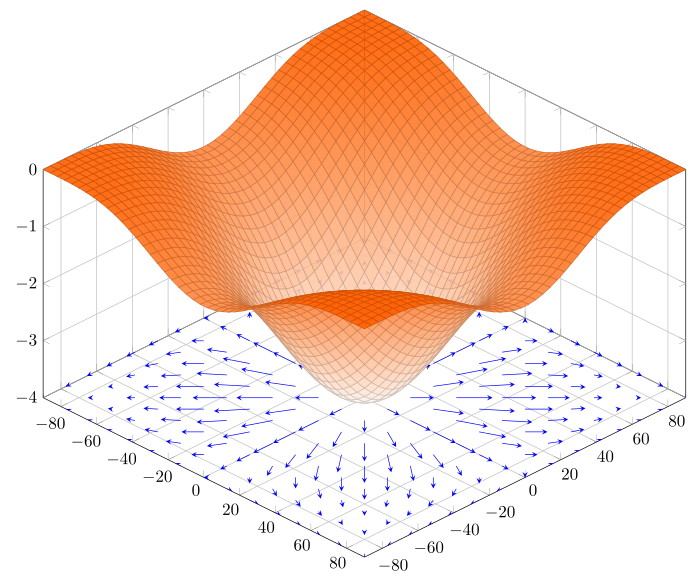
\includegraphics[width=.5\textwidth]{04/grad}
	\caption{The gradient points towards the direction of steepest ascent.}\label{fig:gradient}	
\end{figure}

In fact, it is
\begin{equation}
    \pdv{f}{\vb{v}}(\vb{x}) = \grad f (\vb{x})^{\top} \vb{v} \overbrace{=}^{\mathclap{\text{by definition of dot product}}} \norm{\grad f (\vb{x})} \norm{\vb{v}} \underbrace{\cos(\theta)}_{\mathclap{\text{angle between the gradient vector and the direction vector}}}
\end{equation}
but the direction vector is a unit vector hence its norm is $1$, therefore we end up with
\begin{equation}
    \pdv{f}{\vb{v}}(\vb{x}) = \norm{\grad f (\vb{x})} \cos(\theta)
    \label{eq:4:3:dir_der_grad}
\end{equation}
which means that the directional derivative along a given direction $\vb{v}$ is proportional to the norm (or magnitude, or length) of the gradient vector times the cosine of the angle in between. In particular, it is maximum when $\cos(\theta) = 1$ which is when $\theta = 0$ therefore the two vectors have the same direction, and this means that indeed the gradient vector encodes the direction in which the directional derivative is maximum, i.e. the direction of steepest ascent.

On the other hand the \emph{length} of the gradient vector encodes how much the function increases in the direction of steepest ascent. However, although one can intuitively understand what we mean by length, we have not defined it.

Indeed, when defining what a vector space is, we made no reference to any concept of length, or direction, or orientation whatsoever. However, the Euclidean space $\mathbb{R}^n$ is not just a vector space, but is equipped with additional structures; in particular, it is equipped with a \emph{metric}, and is thus a \emph{metric space}, i.e. it has a notion of \emph{distance} between two points, that actually gives the name to the whole space since it is called the \emph{Euclidean distance}, which is the one we are used to. 

A metric or distance is a function $d(\cdot, \cdot) \to \mathbb{R}$ that tells us how distant two points of a metric space are from each other. One can define any distance, for instance the Euclidean distance is a particular instance of a more general class of distance functions, called $L_p$ distance, which expressed in matrix notation, is:
\begin{equation}
	d(\mathbf{x},\mathbf{y}) = \|\mathbf{x} - \mathbf{y}\|_p \triangleq \left( \sum_{i=1}^{k}|x_i - y_i|^p\right)^{\frac{1}{p}}.
\end{equation}
We can appreciate how setting $p = 2$ in the definition above we recover the usual definition of Euclidean distance, therefore it is also sometimes referred to as $L_2$ distance:
\begin{equation}
    d(\vb{x}, \vb{y}) = \norm{\vb{x} - \vb{y}}_2 = \left( \sum_{i=1}^{k}|x_i - y_i|^2 \right)^{\frac{1}{2}} = \sqrt{(x_1 - y_1)^2 + (x_2 - y_2)^2 + \dots + (x_n - y_n)^2}.
\end{equation}

Once we have a space equipped with a metric, we can measure distances between vectors from that space. With this tool we can define a notion of \emph{length}, or \emph{norm} of a vector as the distance of the vector from the origin:
\begin{equation}
	\|\mathbf{x} - \mathbf{0}\|_2 = \|\mathbf{x}\|_2 = \sqrt{\sum_{i=1}^{k}|x_i|^2} = \sqrt{\mathbf{x}^\top\mathbf{x}};
\end{equation}
we now have a \emph{normed} space, of which the Euclidean space is the most known instance.

So, going back to linear regression, we have that:
\begin{equation}
	\mathbf{\Theta}^* = \argmin_{\mathbf{\Theta} \in \mathbb{R}} \ell(\mathbf{\Theta})
\end{equation}
where 
\begin{equation}
	\ell(a,b) = \sum_{i=1}^{n}(y_i - ax_i - b)^2
\end{equation}
we can see that $\ell$ is a convex function, since a quadratic function is convex and so is the sum of quadratic functions, so we can find the parameters that globally minimize the loss function by setting the gradient equal to $\mathbf{0}$
\begin{align}
	\nabla_{\mathbf{\Theta}}\ell(\mathbf{\Theta}) &= \nabla_{\mathbf{\Theta}}\sum_{i=1}^{n}(y_i - ax_i - b)^2 = \sum_{i=1}^{n}\nabla_{\mathbf{\Theta}}(y_i - ax_i - b)^2 \tag{by linearity of gradient} \\
	&=  \sum_{i=1}^n \nabla_{\bm{\Theta}} (\cancel{y_i^2} + a^2 x_i^2 + b^2 -2a x_i y_i -2by_i +2abx_i) \tag{$\nabla_{\mathbf{\Theta}}y_i^2 = 0$} \\
	&= \sum_{i=1}^n \begin{pmatrix} 2ax_i^2 - 2 x_i y_i + 2bx_i \\ 2b - 2y_i + 2ax_i \end{pmatrix}
\end{align}
where the first element of the vector is the partial derivative with respect to $a$ and the second element is the partial derivative with respect to $b$
\begin{equation}
	\nabla_{\mathbf{\Theta}}\sum_{i=1}^n  ( y_i - a x_i - b )^2 = \begin{pmatrix} \sum_{i=1}^n 2ax_i^2 - 2 x_i y_i + 2bx_i \\ \sum_{i=1}^n 2b - 2y_i + 2ax_i \end{pmatrix}
\end{equation}

Now we can set the gradient equal to zero and solve the system of two linear equation (linear in $a$ and $b$)
\begin{equation}
	\begin{pmatrix} \sum_{i=1}^n ax_i^2 + bx_i  -  x_i y_i  \\ \sum_{i=1}^n ax_i + b - y_i  \end{pmatrix} = \begin{pmatrix}0\\0\end{pmatrix}
\end{equation}

Similarly, in matrix notation we can write all the equations $y_i = ax_i + b$ at once to make the linearity w.r.t. $a,b$ evident:
\begin{equation}
	\underbrace{\begin{pmatrix} y_1  \\ y_2  \\ \vdots  \\ y_n \end{pmatrix}}_\mathbf{y} = \underbrace{\begin{pmatrix} x_1 & 1 \\ x_2 & 1 \\ \vdots & \vdots \\ x_n & 1 \end{pmatrix}}_\mathbf{X}  \underbrace{\begin{pmatrix} a \\ b \end{pmatrix}}_{\bm{\theta}}
\end{equation}

Then, the MSE can be expressed as the $L_2$ distance:
\begin{align}
	\ell(\bm{\theta}) & = \| \mathbf{y} - \mathbf{X} \bm{\theta} \|_2^2 \\
	& = \left( \mathbf{y} - \mathbf{X} \bm{\theta} \right)^\top \left( \mathbf{y} - \mathbf{X} \bm{\theta} \right) \\
	& = \mathbf{y}^\top\mathbf{y} - \vec{y}^\top \vec{X}\bm{\theta} - (\vec{X}\bm{\theta})^\top \vec{y}  +  \bm{\theta}^\top\mathbf{X}^\top \mathbf{X}\bm{\theta}  \\
    & = \mathbf{y}^\top\mathbf{y} -2 \mathbf{y}^\top \mathbf{X}\bm{\theta} + \bm{\theta}^\top\mathbf{X}^\top \mathbf{X}\bm{\theta} \label{eq:lr-norm-eq} 
\end{align}
where in \cref{eq:lr-norm-eq} we used the fact that both $\vec{y}$ and $\vec{X}\bm{\theta}$ are vectors, and the dot product between vector is commutative.

Setting the gradient w.r.t. $\bm{\theta}$ to zero we get
\begin{align}
	-2 \mathbf{X}^\top \mathbf{y}  + 2 \mathbf{X}^\top \mathbf{X}\bm{\theta} = \mathbf{0} \\
	\mathbf{X}^\top \mathbf{X}  \bm{\theta} =  \mathbf{X}^\top\mathbf{y} \\
	\bm{\theta} = (\mathbf{X}^\top \mathbf{X})^{-1} \mathbf{X}^\top\mathbf{y}
\end{align}

In the general case, we have higher-dimensional datapoints:
\begin{equation}
	\mathbf{y}_i = \mathbf{Ax}_i + \mathbf{b} ~~~\mathrm{for~} i=1,\dots,n
\end{equation}
Stacking all data points into matrices $\tilde{\mathbf{X}}=\left(\begin{smallmatrix}|&|&\\\mathbf{x}_1&\mathbf{x}_2&\cdots\\|&|&\end{smallmatrix}\right)$ and $\mathbf{Y}$, we get:
\begin{equation}\label{eq:lin_reg}
	\underbrace{\begin{pmatrix} y_{11} & \cdots & y_{1d}  \\ y_{21} & \cdots & y_{2d}   \\
	 \vdots & & \vdots  \\ y_{n1} & \cdots & y_{nd} \end{pmatrix}}_{\mathbf{Y}^\top} = \underbrace{\begin{pmatrix} x_{11} & \cdots & x_{1d} & 1  \\ x_{21} & \cdots & x_{2d} & 1 \\ \vdots & &\vdots & \vdots  \\ x_{n1} &  \cdots & x_{nd} & 1 \end{pmatrix}}_{\mathbf{X}^\top:=(\tilde{\mathbf{X}}^\top|\mathbf{1})}  \underbrace{\begin{pmatrix} a_{11} & \cdots & a_{1d} \\ \vdots & &\vdots \\ a_{d1} & \cdots & a_{dd} \\ b_1 & \cdots & b_d\end{pmatrix}}_{\bm{\Theta}} 
\end{equation}
where to get the matrix $\mathbf{\Theta}$ we just transposed the vector $\mathbf{b}$ and put it below the matrix $\mathbf{A}$.

According to \cref{eq:lin_reg}, for each output data point $\mathbf{y}_i$ we have:
\begin{equation}
	\underbrace{\begin{pmatrix} y_{i1} \\  \vdots \\ y_{id} \end{pmatrix}}_{\mathbf{y}_i} = \begin{pmatrix} \sum_{j=1}^d a_{j1} x_{ij}  + b_1 \\ \vdots \\  \sum_{j=1}^d a_{jd} x_{ij}  + b_d \end{pmatrix}
\end{equation}

So, the \emph{MSE} becomes
\begin{equation}
	\ell(\bm{\Theta}) = \| \mathbf{Y}^\top - \mathbf{X}^\top\bm{\Theta}\|_2^2 = \mathrm{tr}(\mathbf{Y}^\top\mathbf{Y}) -2 \mathrm{tr}(\mathbf{Y}\mathbf{X}^\top \bm{\Theta}) + \mathrm{tr}(\bm{\Theta}^\top\mathbf{X}\mathbf{X}^\top \bm{\Theta})
\end{equation}